%!TEX root = ../../beamer.tex
\begin{frame}
\frametitle{stochasticity in gene expression}
\begin{center}
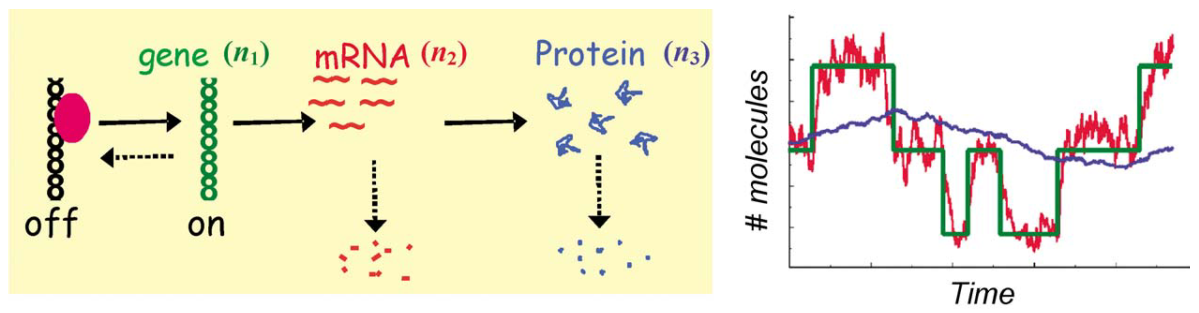
\includegraphics[width=0.9\textwidth]{fig/stochgeneexpdyn.png}\\
{\scriptsize
$n_1$ number of active genes, $n_2$ number of mRNAs, $n_3$ proteins per cell
\begin{align*}
\frac{d \langle n_1 \rangle}{dt} = &\lambda_1^+ (n_1^{max}-\langle n_1 \rangle -\lambda_1^- \langle n_1 \rangle\\
\frac{d \langle n_2 \rangle}{dt} = &\lambda_2 \langle n_1 \rangle -\langle n_2 \rangle / \tau_2\\
\frac{d \langle n_3 \rangle}{dt} = &\lambda_3 \langle n_2 \rangle - \langle n_3 \rangle / \tau_3
\end{align*}}
\end{center}
\end{frame}
